
\section{Bài tập cuối chương}
\begin{multicols}{2}
  \begin{enumerate}

  \item Hãy xác định đầu ra của mỗi mạch sau đây, giả sử đầu vào phía trên là $1$ và đầu
    vào phía dưới là $0$.
    \begin{enumerate}
    \item \scalebox{0.6}{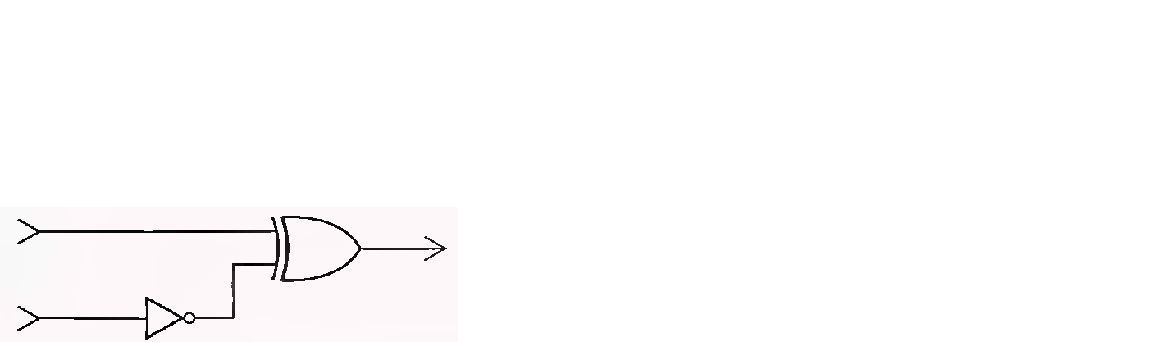
\includegraphics{ch2/ex21a.pdf}}

    \item \scalebox{0.6}{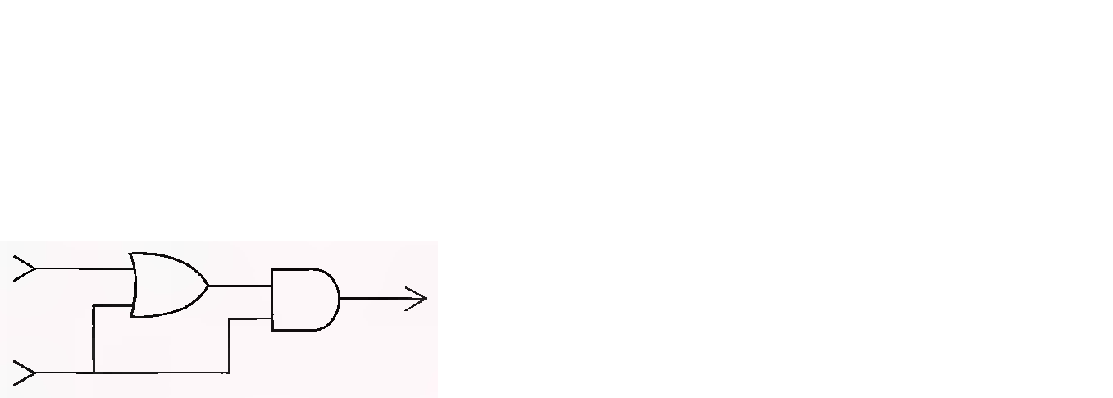
\includegraphics{ch2/ex21b.pdf}}

    \item \scalebox{0.6}{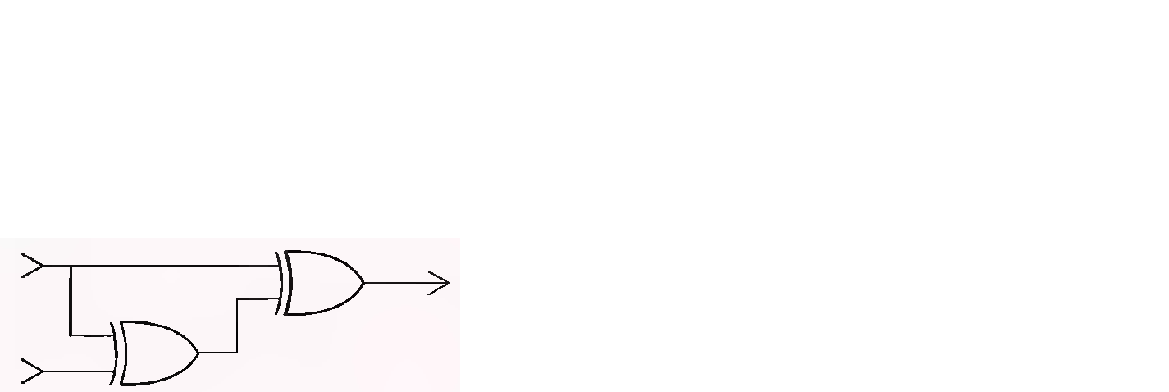
\includegraphics{ch2/ex21c.pdf}}
    \end{enumerate}
  \item Với mỗi mạch dưới đây, hãy xác định các tổ hợp đầu vào để đầu ra là $1$.
    \begin{enumerate}
    \item \scalebox{0.6}{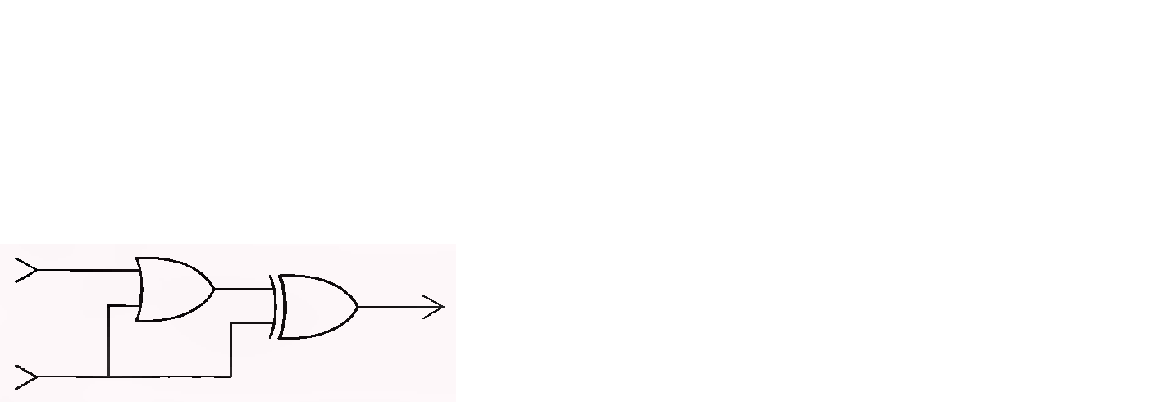
\includegraphics{ch2/ex22a.pdf}}

    \item \scalebox{0.6}{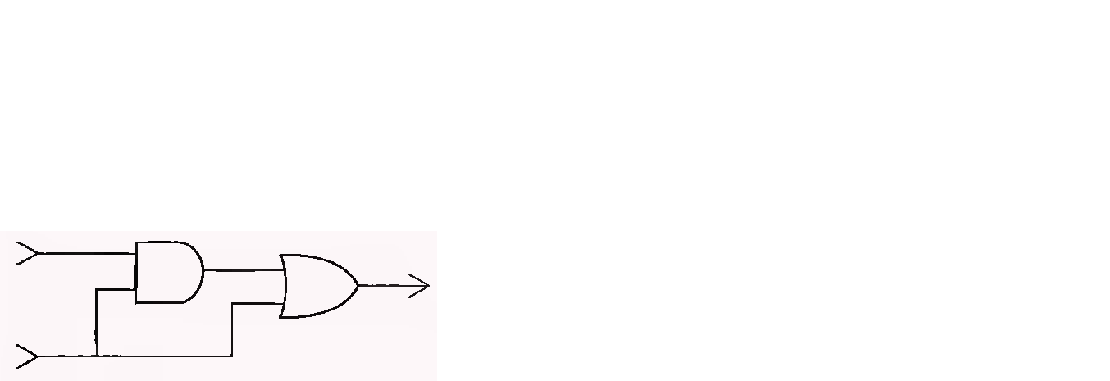
\includegraphics{ch2/ex22b.pdf}}

    \item \scalebox{0.6}{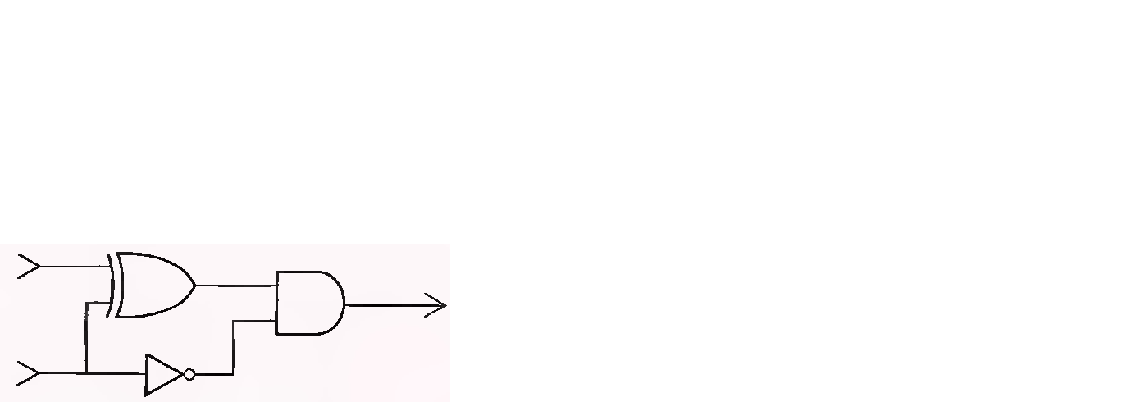
\includegraphics{ch2/ex22c.pdf}}

    \end{enumerate}

  \item Trong mỗi mạch dưới đây, các hình chữ nhật biểu diễn cùng một loại cổng. Dựa vào
    thông tin đầu vào và đầu ra, hãy xác định cổng liên quan trong hình là $\AND$, $\OR$
    hay $\XOR$.
    \begin{enumerate}
    \item \scalebox{0.6}{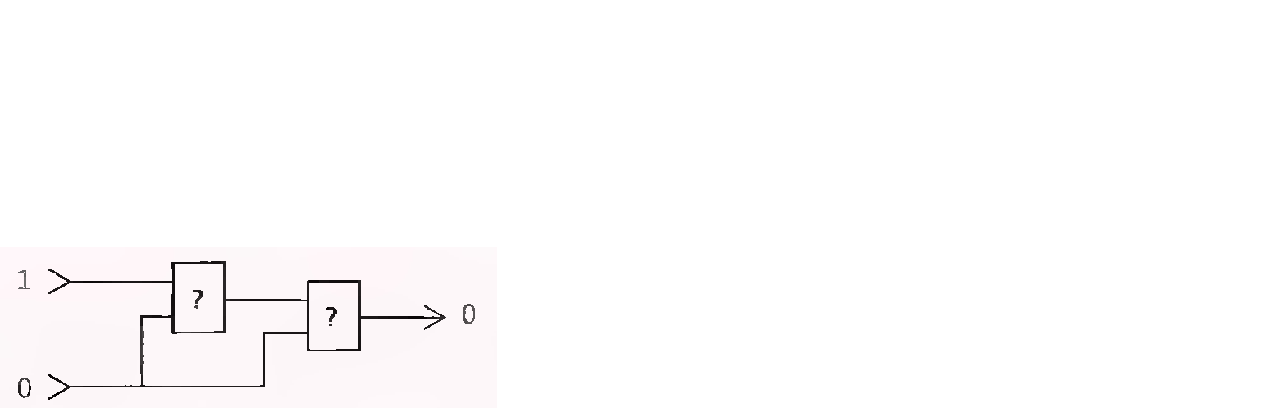
\includegraphics{ch2/ex23a.pdf}}

    \item \scalebox{0.6}{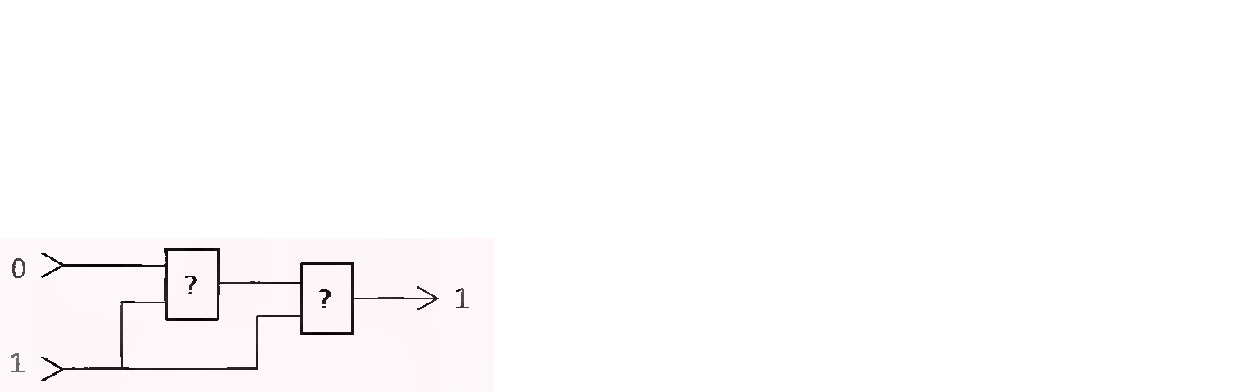
\includegraphics{ch2/ex23b.pdf}}

    \item \scalebox{0.6}{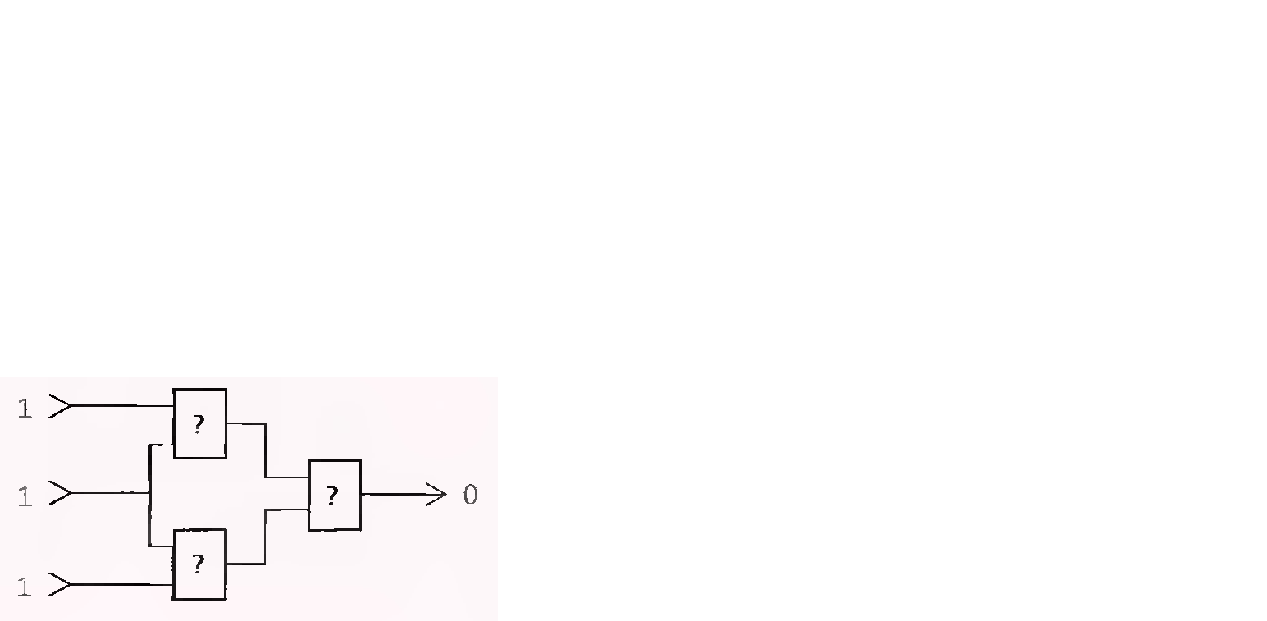
\includegraphics{ch2/ex23c.pdf}}

    \end{enumerate}

  \item Giả sử rằng cả đầu vào và đầu ra trong mạch dưới đây là $1$. Mô tả xem chuyện gì
    xảy ra nếu đầu vào phía trên tạm thời thay đổi về $0$. Mô tả xem chuyện gì xảy ra nếu
    đầu vào phía dưới tạm thời thay đổi về $0$. Vẽ lại mạch sử dụng các cổng $\NAND$.
    \begin{center}
      \scalebox{0.7}{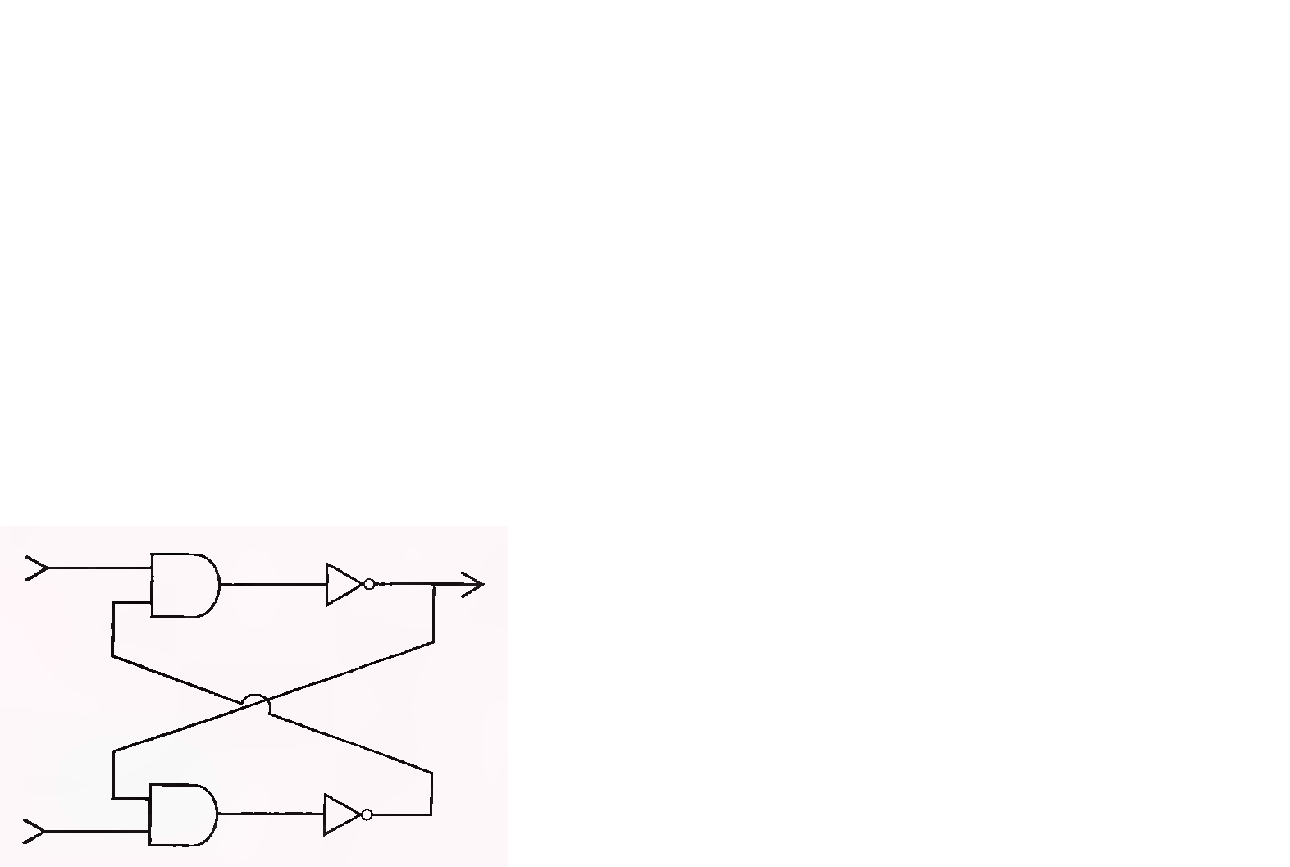
\includegraphics{ch2/ex24.pdf}}
    \end{center}
  \item Bảng dưới đây biểu diễn địa chỉ và nội dung (dùng ký hiệu hexa) của một vài ô nhớ
    trong bộ nhớ chính của máy tính. Hãy thực hiện theo dãy các lệnh ở dưới đây và ghi lại
    nội dung của các ô nhớ này.

    \begin{tabular}[c]{cc}
      Địa chỉ & Nội dung \\
      $00$ & $AB$ \\
      $01$ & $53$ \\
      $02$ & $D6$ \\
      $03$ & $02$
    \end{tabular}
    \begin{enumerate}[B1. ]
    \item Chuyển nội dung của ô nhớ có địa chỉ là $03$ vào ô nhớ địa chỉ~$00$.

    \item Chuyển giá trị $01$ vào ô nhớ tại địa chỉ $00$.

    \item Chuyển giá trị được lưu trữ tại địa chỉ $01$ vào ô nhớ tại địa chỉ~$03$.
    \end{enumerate}

  \item Nếu địa chỉ mỗi ô nhớ của một máy được biểu diễn bởi hai số hexa, vậy có bao nhiêu
    ô nhớ trong bộ nhớ chính của máy tính này?  có bao nhiêu ô nhớ nếu mỗi ô nhớ biểu diễn
    bởi bốn số hexa?

  \item Xâu bít gì được biểu diễn bởi ký hiệu hexa sau đây?

    \begin{inparaenum}[a.]
    \item $CB$ \quad
    \item $67$ \quad
    \item $A9$ \quad
    \item $10$ \quad
    \item $FF$
    \end{inparaenum}

  \item Giá trị của bít trọng số cao nhất trong xâu bít được biểu diễn bởi các ký hiệu
    hexa sau đây là gì?

    \begin{inparaenum}[a.]
    \item $7F$ \quad
    \item $FF$ \quad
    \item $8F$ \quad
    \item $1F$
    \end{inparaenum}

  \item Biểu diễn các xâu bít dưới đây thành ký hiệu hexa:
    \begin{enumerate}[a.]
    \item $101010101010$
    \item $110010110111$
    \item $000011101011$
    \end{enumerate}

  \item Giả sử một camera số có một khả năng lưu trữ là $256$MB. Có bao nhiêu bức ảnh có
    thể được lưu trữ trong camera nếu mỗi ảnh bao gồm $1024$ điểm ảnh trên một dòng và
    $1024$ điểm ảnh trên một cột và nếu mỗi điểm ảnh cần ba byte để lưu trữ.

  \item Giả sử một bức ảnh được biểu diễn trên màn hình máy tính bởi một mảng hình chữ
    nhật chứa $1024$ cột và $768$ dòng điểm ảnh. Nếu tám bít yêu cầu để mã hoá màu và
    cường độ của mỗi điểm ảnh, vậy cần bao nhiêu ô nhớ (tính theo byte) để lưu trữ được
    toàn bộ bức ảnh này.

  \item \begin{enumerate}[a.]
    \item Chỉ ra hai ưu điểm của bộ nhớ chính so với đĩa từ.
    \item Chỉ ra hai ưu điểm của đĩa từ so với bộ nhớ chính.
    \end{enumerate}

  \item Giả sử bạn chỉ còn $50$GB trống trong ổ đĩa cứng $120$GB của bạn. Có hợp lý không
    khi bạn định dùng các đĩa CD để lưu trữ toàn bộ dữ liệu trên ổ như dữ liệu backup? Có
    hợp lý không khi dùng DVD?

  \item Nếu mỗi sector trên đĩa từ chứa $1024$ byte, ta cần bao nhiêu sector để lưu trữ
    một trang văn bản (mỗi trang chứa khoảng $50$ dòng, mỗi dòng khoảng $100$ ký tự) và
    mỗi ký tự được biểu diễn dùng Unicode?

  \item Ta cần bao nhiêu byte để lưu trữ $400$ trang ở đó mỗi trang lưu trữ $3500$ nếu ký
    tự được mã hoá dùng ASCII? Cần bao nhiêu byte nếu mỗi ký tự biểu diễn ở dạng Unicode?

  \item Thời gian trễ của một đĩa cứng là bao nhiêu nếu nó quay với tốc độ $60$ vòng trên
    giây?

  \item Thời gian truy cập trung bình của đĩa cứng là bao nhiêu nếu nó quay với tốc độ
    $60$ vòng trên giây và thời gian dịch chuyển là $10$ milli giây?

  \item Giả sử một người đánh máy có thể đánh được $60$ từ trong một phút liên tục từ ngày
    này sang ngày khác. Để số ký tự đã đánh lưu vào được đầy một đĩa CD kích thước
    $640$MB, người này cần đánh máy trong bao lâu? (giả sử một từ gồm năm ký tự và mỗi ký
    tự cần một byte để lưu trữ.)

  \item Đây là một bức thông điệp ở dạng ASCII. Hãy giải mã xem nó nói
    gì? \\
    \texttt{01010111 01101000 01100001 01110100 00100000 01100100 01101111 01100101
      01110011 00100000 01101001 01110100 00100000 01110011 01100001 01111001 00111111}

  \item Thông điệp dưới đây được mã hoá dưới dạng ASCII dùng một byte cho mỗi ký tự và
    được biểu diễn dùng ký hiệu hexa. Thông điệp sau
    đây muốn nói gì?
    \begin{center}
      $68657861646563696D616C$
    \end{center}
  \item Mã hoá các câu sau đây dưới dạng mã ASCII dùng một byte một ký tự.
\label{ex:221}
    \begin{enumerate}[a.]
    \item $100/5=20$
    \item To be or not to be?
    \item The total cost is \$$7.25$.
    \end{enumerate}
 
  \item Biểu diễn các câu trả lời của bài \ref{ex:221} dưới dạng ký hiệu hexa.

  \item Liệt kê các biểu diễn nhị phân của các số nguyên từ $6$ tới $16$.

  \item \begin{enumerate}[a.]
    \item Viết số $26$ bằng cách biểu diễn $2$ và $6$ ở dạng ASCII.

    \item Viết số $26$ ở dạng biểu diễn nhị phân.
    \end{enumerate}

  \item Những giá trị nào trong biểu diễn nhị phân chỉ có một trong các bít bằng~$1$? Liệt
    kê các biểu diễn nhị phân cho sáu giá trị nhỏ nhất với tính chất này.

  \end{enumerate}

\end{multicols}



%%% Local Variables: 
%%% mode: latex
%%% TeX-master: "../tindaicuong"
%%% End: 
